\chapter{Background}
%-Available spike analysis frameworks \\
%-fieldtrip \\\
%-elephant \\
%-Why they are not sufficient \\
%-problem with the relays? maybe windows updates 

%-openMNGlab as a solution \\
%-acquisition frameworks we need to handle \\
%-Current status of openMNGlab, including Neo \\
%-go into detail on different data acquisition softwares \\
%-Dapsys, OpenEphys, Spike2 \\
%-why does dapsys not work in the future \\

\section{Analysis tools}
When it comes to analysis software for microneurography data,  there are multiple available that each have their own use-cases.

\subsection{FieldTrip}
Fieldtrip (fieldtriptoolboX.org) is a software developed at the Radboud University,  Nijmegen,  the Netherlands and offers a wide variety of analysis functions.  It can analyze MEG, EEG, and other electrophysiological data.

The main problem with this software is its programming language. It is a MATLAB toolbox, however it would be preferred to use a software package in python or another programming language that slots better in the already existing structure within the chair for medical informatics. In addition to that it is not only speficied for spike trains software, dealing with MEG, EEG and iEEG analysis. 

\subsection{Elephant}
Elephant (https://elephant.readthedocs.io/en/latest/index.html) is a python module which offers some high-level analysis functions for spike trains specifically.  The main problem with this software is the lack of basic functionalities.  It relies more on highly specified analysis tools that are not necessarily viable in our use-case.  For the use in this thesis I want to start with the basic signal from the spikes, try out different quantifiers and look at the data from a fresh perspective. 

\subsection{openMNGlab}
These are two analysis tools I presented that could not be used for this thesis  because of different reasons.
There are multiple data acquisition software solutions that are used at the chair of IMI that each produce different file formats.. The three main acqusition software packages that need to be handled are Spike2, Dapsys and OpenEphys and are described in more detail in the next section. \\ 
We need a tool that that has the capability to load files from these different data acqusition softwares, put them in a compatible format and analyze them further.  FieldTrip does not offer these kinds of capabilities as well as it being a matlab package, which would not be ideal for fitting into the rest of the analysis systems at IMI. Elephant is also lacking the importing tools that would be required for the software solution.  \\
For this reason the Institute of medical informatics has started to develop their own software framework in python called openMNGlab.  This framework aims to provide a solution for those issues with the different file types and combine them into a single usable format.  In addition it provides analysis capabilities for microeurography data. \\
For the import of the different file types from the data acqusition packages and the internal structure of the data openMNGlab makes use of an already developed python module called Neo(neuralensemble.org/neo). This is a package that already deals with neurophysiological data in various different file formats. It is aimed towards combining these different sources while not providing any analysis capabilities of its own to reduce dependencies (cite website here). It also comes with templates to build importers for different new file formats should those be required and thus makes it easier to include more file formats at a later date.\\
OpenMNGlab has started as a project of the Institute of medical informatics and was initially developed by Fabian Schlebusch who developed openMNglab 1.0 and setup the basic structure and developed the importers necessary for the file formats that we require. \\
However, the 1.0 version of the framework is not enough in terms of analysis and also importing capabilities and needs to be improved. 

At IMI there are people who work on varying aspects of MNG data analysis such as analyzing the response latency to electrical stimulation or analyzing the nerve activity in response to certain chemicals. I am focusing on analyzing spike trains occuring in mechanically and electrically stimulated nerve fibers.\\
With my bachelor thesis I aim to provide some more analysis functionalities for spike trains as well as give some ideas on the software engineering of the software framework in the future.\\
In the end FieldTrip and Elephant offer good solution for slightly different use-cases, but were not a perfect fit for the analysis of microneurography data at the Institute of medical informatics. They are, however, a good inspiration for what should be included in such a software framework. In the case of Elephant, since it is also a python module and also makes use of the Neo structure, it could make for a good addition of more high-level analysis functionalities in the future.



Neo:\\
brings a data structure\\
importers or at least templates for importers



\section{Data acquisition software} 
A data acqusition system is a combination of software and hardware components that offer the ability to control and record physical aspects of something.%TODO: find better wording for this
There are many different data acquisition systems for electrophysiological data. There are three systems that we are working with and that should be comaptible with our chosen software analysis framework. These systems are Spike2, Dapsys and OpenEphys.

\subsection{Spike2}
%“Spike2 is a multi-channel continuous data acquisition and analysis package”( https://ced.co.uk/products/spkovin) produced by Cambridge electronic design limited. \\
%-Used for the experiments I am analysing by Roberto \\
%-records data in multiple channels \\
%-channel for raw signal \\
%-channel for mechanical force \\
%-channel for event markers \\
%-channel for temperature (not used by me) \\
%-channel for comments (used for marking when chemicals are applied) \\
%-spikes can be separated into own channels (done by experimenters) \\
%-software offers a graphical representation of the data \\
%-channels are separated \\
%-was used for confirmation of what the data should output in terms of basic quantifiers \\
%-can export csv files from the data \\
%-has direct importer in openMNGlab \\

Spike2 is a data acquisition and analysis software produced by Cambridge electronic design limited. It is a flexible tool that can be used in a variety of different ways.

TODO: go into detail\\

\begin{figure}
	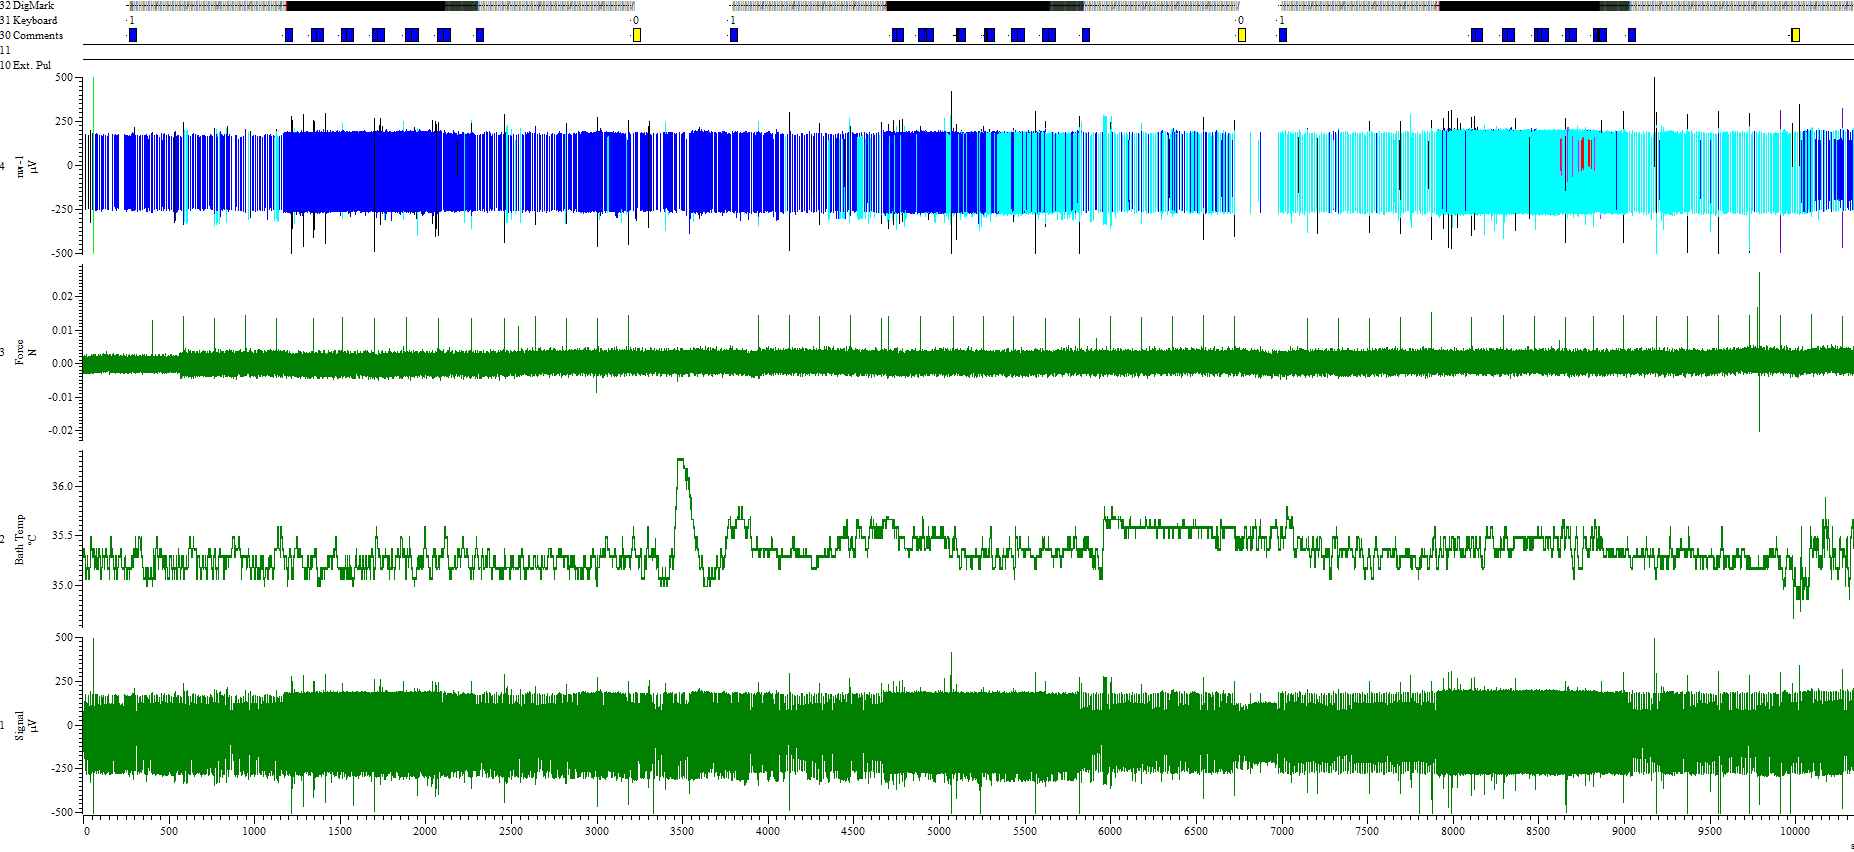
\includegraphics[width = \textwidth]{src/pic/Spike2_screenshot}
	\caption{Typical mechanically and electrically stimulated recording in Spike2}
	\label{fig:spike2}
\end{figure}

The software can record multiple channels simultaneously. An example screenshot from a recording can be seen in Figure~\ref{fig:spike2}. This depicts a typical recording used for analysis in this bachelor thesis. The recording contains data from nerve fibers of rat cranial dura mater. The nerve fibers were stimulated using a mechanoelectrostimulator applying electaical and mechanical stimulation. 

\begin{figure}
	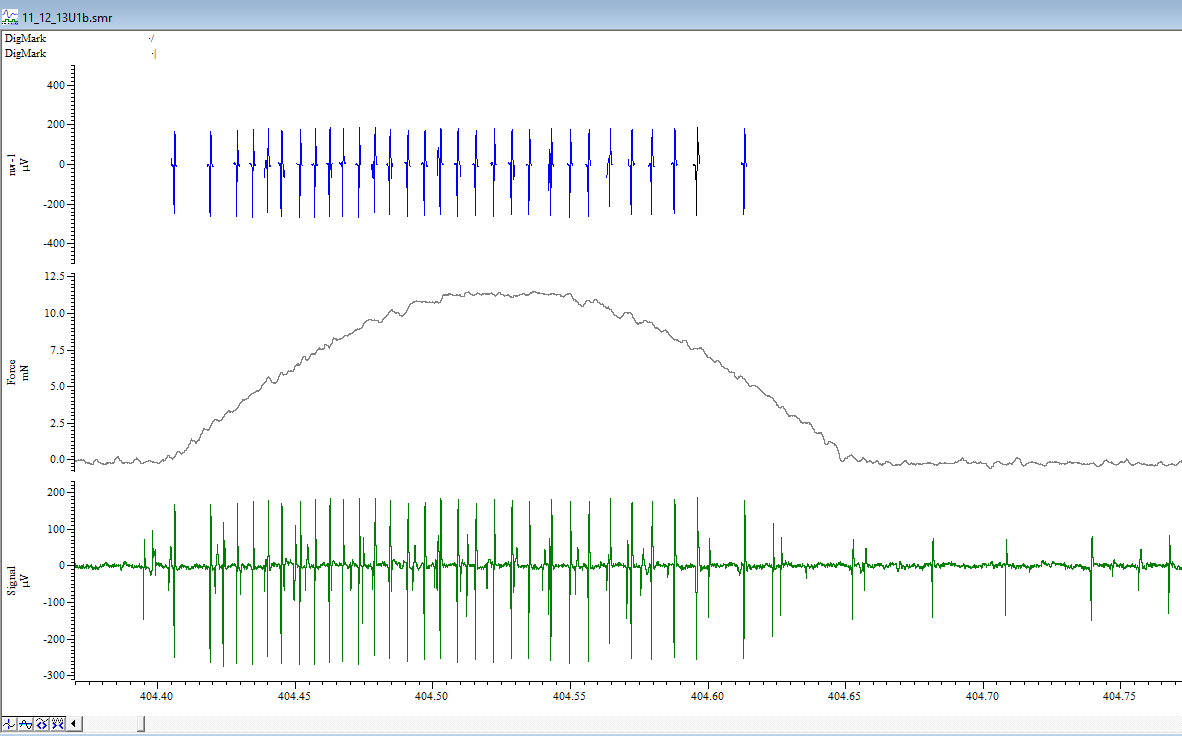
\includegraphics[width = \textwidth]{src/pic/Spike2_spike_train}
	\caption{A single spike train in spike2}
	\label{fig:spike_train}
\end{figure}

First of all it contains a channel for the recorded raw signal at the bottom. The next channel contains the temperature during the recording. In this example it fluctuates between 35°C and 36.5°C. In channel 3 we can observe the mechanical force that was applied to the nerve fibers. In Figure~\ref{fig:spike2} there are spikes in mechanical force whenever a mechanical stimulation occurs to evoke a spike train. For this experiment we want to collect the data of single nerve fibers. It is diffucult, to record just a single nerve fiber in vitro, however. This is why in this experiment spike templates are applied to the raw signal to filter out specific fibers. These filtered fibers are then displayed in so called wavemark channels. In this example channel 4 is such a channel, where only specific action potentials are filtered. The filtering process is done by the experimenters and is based on certain features of the action potential shape.\\
The topmost channel in Figure~\ref{fig:spike2} contains markers for the electrical and mechanical stimuli. Additionally there is a channel containing comments regarding the experiment. Comments can represent the experimental protocol and are filled in by the experimenters. In this example there are comments denoting a change electrical stimulation frequency. In other experiments for example, these could also denote the application of certain chemicals towards the recorded subject.

A more detailed view of a single spike train can be seen in Figure~\ref{fig:spike_train}. Here the difference in electrical and mechanical event markers in the topmost channel can be seen. Mechanical markers are represented by a slash, while electrical markers are represented by a vertical line. Another thing that can be seen here is the channel containing only the spikes. This channel is ideal for the extraction of the spikes for later analysis as there is no noise in the channel anymore and the spikes can also be interpreted as simple events with a timestamp.

\subsection{Dapsys}
%“DAPSYS is a combined hardware and software system designed for real-time acquisition and display of data and synchronous %control of stimulators.” (http://www.dapsys.net/) \\
%-Used by Barbara for her experiments \\
%-used for mng-experiments with human patients \\
%-also has a graphical representation of the data \\
%-has importer in openMNGlab \\
%-needs to export specific templates as csv for the importer to work \\
%-Dapsys has problem in the future \\
%-it gets harder to set up experimental protocols \\
%-maybe it has something to do with newer windows updates \\
%-that means this will probably not be used much in the future \\
%http://www.dapsys.net/rd_article/rd_article.html

The second data acquisiton package that openMNGlab needs to support is called Dapsys. It is a hardware and software system that can record and analyze electrophysiological data from animal or human sources and has been mainly used for studying the peripheral nervous system (cite website here). It has been in development for over 30 years since its earliest version. \\
Dapsys offers the capabilities of path tracking and comes with the benefit of much data being available from experiments conducted with the Dapsys software. It is used especially for mng-experiments with human patients. As is the case for Spike2 it also comes with a visual representation of the data which can be seen in Figure~(put ref to screenshot here). This graphical interface works real time while recording the data.\\
The version of Dapsys used in the experiments from Barbara Namer is specialized for microneurography and was configured in cooperation with Brian Turnquist.\\
The data can also be imported by openMNGlab, however, unlike Spike2, where we can directly import the experimental file, we first need to do an extra step. We need to export the raw data and templates for the tracks we want to analyze as csv files from the Dapsys software.\\


\subsection{OpenEphys}
%OpenEphys \\
%-open-source electrophysiology \\
%-based in Cambridge, Massachusetts \\
%-Used in experiments in Bristol cooperation \\
OpenEphys is an open-source electrophysiology data acqusition software from a nonprofit based in Cambridge, Massachusetts. Its aim is that in the future neuroscientists can choose the right tool for their job and that there are many tools available. This is best accomplished by providing open-source solutions.
OpenEphys is used by one of the collaborators of IMI in Bristol.

 
\cleardoublepage
